\documentclass[10pt,pra,aps,twocolumn,superscriptaddress,floatfix,nofootinbib]{revtex4-2}
\usepackage[T1]{fontenc}
\usepackage{newtxtext,newtxmath}
\usepackage{graphicx}
\usepackage{booktabs}
\usepackage{xcolor}
\usepackage{microtype}
\usepackage{tikz}
\usetikzlibrary{arrows.meta,positioning,calc}
\usepackage[colorlinks=true,linkcolor=linkblue,citecolor=linkblue,urlcolor=linkblue]{hyperref}

\definecolor{linkblue}{HTML}{1C5CAB}
\definecolor{learn}{HTML}{2A78D6}
\definecolor{ink}{HTML}{52514E}
\definecolor{gls}{HTML}{EB6834}

\newcommand{\GLS}{GLS}
\newcommand{\emumps}{EMU\_MPS}
\renewcommand{\arraystretch}{1.12}

\begin{document}

\title{Learned piece selection for divide-and-conquer maximum independent set on neutral-atom arrays}

\author{Hamzah Azzam}
\email{azzam1@stolaf.edu}
\affiliation{Department of Mathematics, Statistics and Computer Science, St.~Olaf College, Northfield, Minnesota 55057, USA}

\date{\today}

\begin{abstract}
Rydberg atom arrays solve the maximum independent set problem natively, but only on small unit-disk graphs. For larger arbitrary graphs, Cazals \textit{et al.} [Phys.\ Rev.\ A \textbf{112}, 062416 (2025)] proposed a divide-and-conquer heuristic that repeatedly cuts out a piece that fits a fixed atom layout, solves it on the processor, and removes the solution and its neighbours. Fixed greedy rules decide how pieces are grown, which are solved, and which partial solutions are kept. We replace these rules with learned models. On 520 fresh instances that no model was trained, tuned or selected on, the best models lower the mean gap to the best known solution from $14.4\%$ to about $2\%$ on graph families seen in training and from $5.8\%$ to about $1\%$ on held-out families, and a tree-search variant does so with fewer quantum runs than the original rules. The gains hold when every piece is sampled from Pasqal's \emumps{} emulator. Two controls limit what this means: a classical minimum-degree greedy heuristic, which uses no quantum runs, does about as well, and random bitstrings with classical repair do about as well as the emulator, because most pieces have fifteen atoms or fewer. Learning improves the decomposition itself, but gives no evidence of a quantum advantage at these sizes.
\end{abstract}

\maketitle

\section{Introduction}

Two neutral atoms closer than the blockade radius cannot both be excited to a Rydberg state. An array of atoms therefore encodes the maximum independent set (MIS) problem on the unit-disk graph defined by the atom positions, and a slow drive prepares a state whose measurement returns large independent sets~\cite{pichler2018quantum,henriet2020quantum,ebadi2022quantum}. Most graphs are not unit-disk graphs. Gadget reductions can embed them exactly~\cite{nguyen2023quantum}, but Cazals \textit{et al.}~\cite{cazals2025gadgets} proved that, under the exponential-time hypothesis, such reductions need quadratically many vertices, and that they cannot preserve approximation ratios unless P${}={}$NP. Instead, they proposed a divide-and-conquer heuristic built on Greedy Lattice Subgraph (\GLS{}) mapping: grow a piece of the graph that fits a calibrated triangular layout, solve its MIS on the processor, remove the solution and its neighbours, and repeat, with a small beam search over pieces and solutions.

Every decision in this loop is made by a fixed rule. A degree-based score orders vertices during growth, the largest pieces are solved, and branches are kept by the size of their partial solution. We ask whether models trained on generated instances make better decisions, measured by the gap to the optimum and by the number of quantum runs a decomposition uses. Much work on learned combinatorial optimization trains a model to build the solution itself~\cite{khalil2017learning,li2018combinatorial,ahn2020defer}. Here the model only chooses what the quantum solver is asked to solve. Garrigues \textit{et al.} applied the same heuristic to molecular docking~\cite{garrigues2025docking}, and other hybrid methods choose the subgraph a neutral-atom sampler solves with classical rules, for example from a linear-programming relaxation~\cite{perron2026lpquts}. The closest learned approaches we know of learn graph partitions for gate-based QAOA~\cite{zheng2026neuralqaoa} or variable elimination in recursive QAOA~\cite{patel2022rlrqaoa}; neither involves an atom layout.

We find that learned decisions cut the gap of \GLS{} by a factor of six to seven on fresh instances, that the improvement survives quantum-sampled answers from Pasqal's emulator, and that at the sizes studied the decomposition does at best slightly better than a classical greedy heuristic while the quantum step does no better than random sampling. The first of these agrees with reports that classical baselines are hard to beat for learned MIS solvers~\cite{bother2022wrong}. The contribution is a better way to run the decomposition, which would matter most where the quantum piece solver is expensive and hard to replace.

\section{The decomposition}
\label{sec:decomposition}

We use the layout and blockade radius of Pasqal's public \GLS{} code~\cite{garrigues2025docking}: 61 traps on a triangular lattice with $5\,\mu$m spacing and a blockade radius of $6.6\,\mu$m, so only nearest neighbours interact (Fig.~\ref{fig:piece}). A \emph{piece} maps some graph vertices to traps so that two vertices are adjacent in the graph exactly when their traps are neighbours. Every piece in this paper passes this check, and every piece sent to the emulator (Sec.~\ref{sec:emulator}) was built as a Pulser register~\cite{silverio2022pulser} on the device's calibrated layout.

\begin{figure*}[t]
\centering
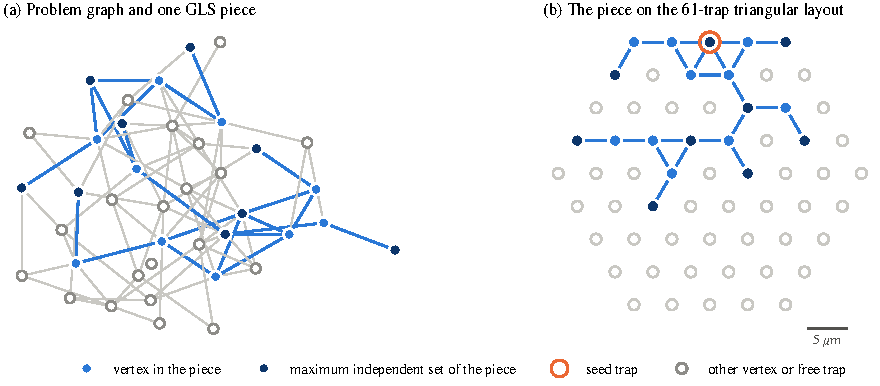
\includegraphics[width=\textwidth]{figures/piece.pdf}
\caption{A piece grown by \GLS{} on an Erd\H{o}s--R\'enyi graph with $n=40$ and $p=0.1$. (a) The 19 vertices of the largest piece (blue) and the 9 vertices of its maximum independent set (dark). Committing this set removes 31 of the 40 vertices. (b) The same piece on the 61-trap layout; graph edges coincide with neighbouring occupied traps. The circled trap is where Pasqal's code places the first vertex.}
\label{fig:piece}
\end{figure*}

A branch is a remaining graph $H$ and a partial independent set $S$, starting from the full graph and the empty set. In each round, every branch grows candidate pieces, up to $k$ of them are solved, each of the $s$ best solutions $T$ of a solved piece (one for pieces of five vertices or fewer) gives a child branch $(H \setminus N[T],\, S \cup T)$, and the beam is pruned (Fig.~\ref{fig:loop}). A branch with five vertices or fewer left is finished by brute force. The models replace four decisions:

\begin{itemize}
\setlength{\itemsep}{1pt}
\item[H2] the order in which neighbours are tried while a piece grows; \GLS{} uses the score $1 - |5 - \deg(v)|/n$, where 5 is the layout's mean degree, 5.11, rounded down;
\item[H3] which trap each vertex goes on; \GLS{} puts each new vertex on the first free trap beside its placed neighbour that keeps the piece valid;
\item[H4] which candidate pieces to solve; \GLS{} takes the $k$ largest;
\item[H5] which branches survive pruning; \GLS{} keeps the largest partial solutions.
\end{itemize}

\begin{figure}[t]
\centering
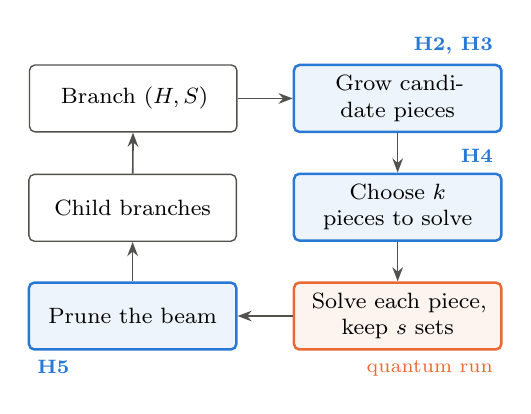
\begin{tikzpicture}[
  font=\footnotesize,
  box/.style={draw=ink, rounded corners=2pt, align=center, minimum height=8.5mm, text width=24mm, fill=white, line width=0.5pt},
  hook/.style={box, draw=learn, fill=learn!8, line width=0.9pt},
  q/.style={box, draw=gls, fill=gls!8, line width=0.9pt},
  arr/.style={-{Stealth[length=1.8mm]}, ink, line width=0.6pt},
  tag/.style={font=\scriptsize\bfseries, text=learn}]
\node[box] (br) {Branch $(H,S)$};
\node[hook, right=7mm of br] (grow) {Grow candidate pieces};
\node[hook, below=5mm of grow] (pick) {Choose $k$ pieces to solve};
\node[q, below=5mm of pick] (solve) {Solve each piece, keep $s$ sets};
\node[hook, left=7mm of solve] (prune) {Prune the beam};
\node[box, above=5mm of prune] (child) {Child branches};
\draw[arr] (br) -- (grow);
\draw[arr] (grow) -- (pick);
\draw[arr] (pick) -- (solve);
\draw[arr] (solve) -- (prune);
\draw[arr] (prune) -- (child);
\draw[arr] (child) -- (br);
\node[tag, anchor=south east] at (grow.north east) {H2, H3};
\node[tag, anchor=south east] at (pick.north east) {H4};
\node[tag, anchor=north west] at (prune.south west) {H5};
\node[font=\scriptsize, text=gls, anchor=north east] at (solve.south east) {quantum run};
\end{tikzpicture}
\caption{One round of the decomposition. Blue boxes are the decisions replaced by learned models; the orange box is the only step that uses the quantum processor.}
\label{fig:loop}
\end{figure}

Pasqal's code differs from the published description in a few ways (Appendix~\ref{app:code}). The main one is that it grows a piece from every vertex and solves the $k$ largest, instead of growing $k$ pieces from random seeds. We follow the code. Given Pasqal's own piece solver, our reimplementation reproduces its output exactly on 96 Erd\H{o}s--R\'enyi test cases. The code's beam can grow without bound on sparse graphs, so all methods, \GLS{} included, run in a bounded version in which the children of small pieces also count toward the pruning trigger $\ell$ (Appendix~\ref{app:code}); a run that exceeds 1000 branches is aborted, which no reported run of this version did.

\textit{Cost.} We count one \emph{quantum run} for every piece a method solves, including pieces of five vertices or fewer, which Pasqal's code solves classically, and for every remainder of five vertices or fewer finished by brute force; otherwise a method could lower its count by aiming for small pieces. We also report \emph{piece-solver runs}, which follow Pasqal's convention and count only larger pieces. As a design rule, no method computes an independent set of a candidate outside a counted solve; the one exception is a reference run that prunes with exact values, labelled as such in Sec.~\ref{sec:results}.

\textit{Piece solvers.} For training and most evaluation, a classical stand-in returns the $s$ largest distinct maximal independent sets of a piece using CP-SAT~\cite{ortools}, the first being a maximum one. For quantum solves, each sampled bitstring is repaired into a maximal independent set, by removing the vertex with most conflicts and then adding vertices in order of increasing degree, and the $s$ most frequent sets are returned.

\section{Learned models}
\label{sec:models}

We built the models roughly in order of cost. Five ideas carry the results.

\textit{Labels.} For a remaining graph $H$ and a candidate piece $P$, the label is the best final size reachable after solving $P$,
\begin{equation}
Q^*(P) = \max_{T} \bigl[\, |T| + \alpha(H \setminus N[T]) \,\bigr],
\label{eq:q}
\end{equation}
where $T$ ranges over the sets the piece solver returns for $P$ and $\alpha$ is the independence number, computed exactly by CP-SAT. H2 rankers are trained instead on whether a vertex belongs to a maximum independent set of $H$. Training states are taken from the graphs the \GLS{} beam visits on training instances; DAgger-trained models also use states visited by the learned policy.

\textit{Rankers} (H2, H4). A ridge regression on nine vertex features or thirteen piece features (degrees, core numbers, piece size and density, the share of $H$ in the piece's closed neighbourhood), fitted within each state so that only the order matters. We also tried graph neural networks (GIN, GraphSAGE and GAT, three layers of width 64~\cite{xu2019gin,hamilton2017sage,velickovic2018gat}) trained with a listwise loss.

\textit{Value-to-go} (H5). A graph network predicts $\alpha(H)$, and branches are pruned by $|S| + \hat\alpha(H)$, the predicted final size, instead of $|S|$.

\textit{Piece builder} (H3). Instead of growing pieces by a vertex order, a network scores every feasible (vertex, trap) pair and places the best one until none is left. Masking guarantees a valid piece. It is trained to imitate growth driven by the DAgger-trained GIN ranker for H2 and then improved with REINFORCE~\cite{williams1992reinforce}.

\textit{Tree search.} A PUCT search~\cite{silver2017mastering} explores pieces in H4 order, guided by $|S| + \hat\alpha(H)$, and stops searching after a budget $B$ of quantum runs; the final descent to a complete solution can spend more, so mean runs slightly exceed $B$ (Table~\ref{tab:fresh}).

We also tested gradient-boosted rankers~\cite{ke2017lightgbm}, a \GLS{}-style score with its target degree and two added terms tuned by CMA-ES~\cite{hansen2001cma}, DAgger relabelling of the policy's own states~\cite{ross2011dagger}, policy gradient with a cost per quantum run, self-play training of the search prior, a GFlowNet builder~\cite{bengio2021gflownet}, and a bandit that picks $k$, $s$ and the beam width each round. Table~\ref{tab:ladder} lists them. Below, \emph{linear + value} is the linear rankers with a GraphSAGE value model, \emph{builder} is the piece builder with DAgger-trained GIN models for H4 and H5, and \emph{builder + search} is the builder inside the tree search at $B=100$. All models were trained on CPUs in hours.

\section{Experimental protocol}
\label{sec:protocol}

The training families are Erd\H{o}s--R\'enyi graphs ($p = 0.1, 0.25, 0.75$), Barab\'asi--Albert graphs ($m = 2, 8$), a four-block stochastic block model, and correlation graphs from a simulated market model ($\theta = 0.2, 0.3$). The held-out families, never trained on, are random geometric graphs (radius $0.10$, $0.15$) and a ``crisis'' market model with twice the market factor ($\theta = 0.3, 0.4, 0.5$). Models train at $n = 60$, 100 and 150 and are tested at $n = 100$ and 150.

Instances are split by random seed into training, validation, selection, test and \emph{fresh} sets. No training, tuning or model selection read the fresh set, which has 320 instances from training families and 200 from held-out ones; headline numbers use it. The model comparisons of Table~\ref{tab:ladder} use the test set.

The gap is $100\,(\alpha^\star - |S|)/\alpha^\star$, where $\alpha^\star$ is the best size found by any method, including CP-SAT with a 120\,s limit, which proves optimality on 479 of the 520 fresh instances. Because a method can trade gap for runs, we compare curves of mean gap against mean quantum runs over widths $(k,s,\ell)$ from $(1,1,1)$ to $(8,3,30)$, where $(4,2,10)$ is the setting of Ref.~\cite{cazals2025gadgets}. Comparisons against a curve use $\Delta$, the method's mean gap minus the curve's gap at the same number of runs. Intervals are $95\%$ bootstrap intervals over instances.

The classical reference is min-degree greedy: repeatedly take a vertex of lowest degree and delete its neighbours, keeping the best of 20 random tie-breaks. It uses no quantum runs and takes 0.15\,s per instance on average.

\section{Results}
\label{sec:results}

\begin{figure*}[t]
\centering
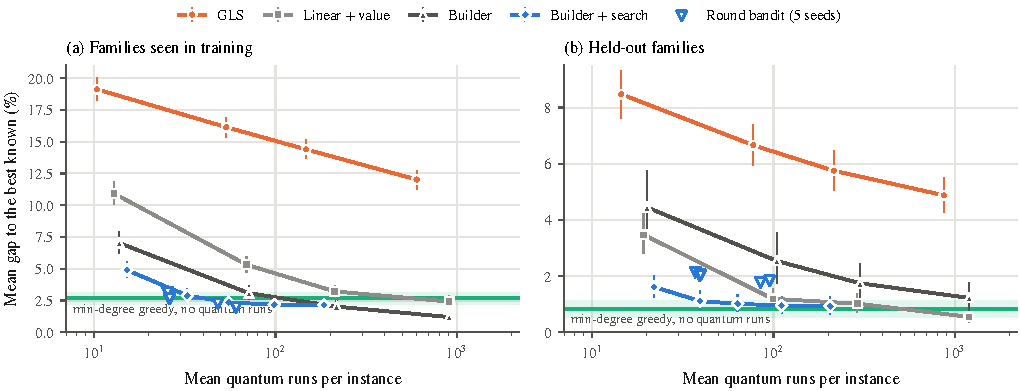
\includegraphics[width=\textwidth]{figures/tradeoff.pdf}
\caption{Mean gap against mean quantum runs on the 520 fresh instances. Each curve sweeps the widths, or the budget $B$ from 6 to 200 for builder + search. Bars are $95\%$ bootstrap intervals. Open triangles are the round bandit trained from five seeds. The green band is min-degree greedy.}
\label{fig:tradeoff}
\end{figure*}

\begin{table*}[t]
\caption{Fresh instances at each method's headline setting, widths $(4,2,10)$ or budget $B=100$. Gap in percent with its $95\%$ interval; $Q$ is mean quantum runs and $P$ mean piece-solver runs per instance. Bold marks the lowest learned gap in each column.}
\label{tab:fresh}
\begin{ruledtabular}
\begin{tabular}{lcrrcrr}
 & \multicolumn{3}{c}{Training families (320 instances)} & \multicolumn{3}{c}{Held-out families (200 instances)} \\
\cline{2-4}\cline{5-7}
Method & Gap (\%) & $Q$ & $P$ & Gap (\%) & $Q$ & $P$ \\
\hline
\GLS{} & 14.39\,[13.67, 15.16] & 147 & 22 & 5.75\,[5.06, 6.48] & 215 & 32 \\
Linear + value & 3.21\,[2.74, 3.70] & 212 & 73 & 1.02\,[0.71, 1.37] & 290 & 86 \\
Builder & \textbf{2.02}\,[1.60, 2.49] & 217 & 85 & 1.74\,[1.17, 2.43] & 300 & 71 \\
Builder + search & 2.17\,[1.74, 2.64] & 98 & 39 & \textbf{0.95}\,[0.68, 1.28] & 111 & 29 \\
\hline
Min-degree greedy & 2.67\,[2.20, 3.17] & 0 & 0 & 0.83\,[0.53, 1.15] & 0 & 0 \\
\end{tabular}
\end{ruledtabular}
\end{table*}

\subsection{Fresh instances}

At the published widths \GLS{} has a mean gap of $14.4\%$ on training families and $5.8\%$ on held-out ones (Fig.~\ref{fig:tradeoff}, Table~\ref{tab:fresh}). Every learned method lies far below the \GLS{} curve at every budget; even with 600 quantum runs, \GLS{} stays at $12.0\%$. The builder reaches $2.0\%$ on training families, and builder + search reaches $0.95\%$ on held-out families with half the quantum runs of \GLS{}.

The saving in runs depends on how they are counted. Most of the quantum runs of \GLS{}, 126 of 147 on training families, are pieces or remainders of five vertices or fewer, which Pasqal's code solves classically. Counting only larger pieces, builder + search sends 39 per instance against 22 for \GLS{}, although the pieces of \GLS{} are bigger.

Min-degree greedy reaches $2.7\%$ and $0.8\%$ with no quantum runs. Compared instance by instance, the builder and builder + search beat it slightly on training families, by 0.65 points ($[0.17, 1.19]$) and 0.50 points ($[0.01, 1.01]$), while on held-out families greedy is level with builder + search and better than the builder by 0.91 points ($[0.31, 1.61]$). Greedy is strong when degrees are recomputed after each removal: on the test seeds, the greedy routine in Pasqal's repository, which sorts vertices by degree once, has gaps of $11.7\%$ and $3.3\%$.

\subsection{What each model contributes}

\begin{table}[t]
\caption{The models on the test seeds, widths $(4,2,10)$ unless a budget is given. Gap in percent on training (Tr) and held-out (Ho) families; $Q$ is mean quantum runs on training families.}
\label{tab:ladder}
\begin{ruledtabular}
\begin{tabular}{lrrr}
Method & Tr & Ho & $Q$ \\
\hline
\GLS{} & 14.15 & 6.09 & 154 \\
\GLS{}, CMA-ES-tuned score & 11.03 & 3.91 & 143 \\
LightGBM ranker, H2 + H4 & 8.74 & 2.67 & 184 \\
Linear ranker, H2 & 9.31 & 3.22 & 142 \\
Linear ranker, H2 + H4 & 7.79 & 2.47 & 183 \\
\quad + value (H5) & 3.51 & 0.71 & 213 \\
GIN, H2 + H4 + H5, after DAgger & 2.68 & 1.27 & 219 \\
\quad with policy-gradient H4 & 2.43 & 1.26 & 173 \\
Builder & 1.98 & 1.34 & 219 \\
GFlowNet builder & 2.36 & 0.66 & 216 \\
Builder + search, $B=100$ & 2.08 & 0.54 & 98 \\
Round bandit & 2.73 & 0.94 & 26 \\
\hline
Min-degree greedy & 3.21 & 0.72 & 0 \\
\end{tabular}
\end{ruledtabular}
\end{table}

Table~\ref{tab:ladder} shows the models in the order they were built. Three changes do most of the work.

The first is the growth order. A linear ranker for H2 lowers the gap from $14.2\%$ to $9.3\%$. Tuning the weights of the \GLS{} score with CMA-ES reaches only $11.0\%$, so the fixed score is not just mistuned; it looks at the wrong quantities.

The second, and largest, is pruning by predicted final size. It lowers the gap of the linear rankers from $7.8\%$ to $3.5\%$ ($\Delta = -4.0$, $[-4.5, -2.8]$) and from $2.5\%$ to $0.7\%$ on held-out families. On the 40 validation instances, pruning with the exact $\alpha$ instead of the prediction changes $\Delta$ by only 0.03 points, so the value model captures almost all of the possible gain.

The third is the piece builder. At equal widths, where both use nearly the same number of runs, it lowers the gap of the DAgger-trained GIN models by a further 0.70 points on training families ($[-1.14, -0.26]$). Inside the tree search it gets the same quality with fewer than half the runs. Graph networks gave little over linear rankers for H2 and H4, and LightGBM, the GFlowNet builder and the bandit gave no reliable gain: the bandit uses few runs, but its result changes with the training seed.

\subsection{Graph families and size}

\begin{figure}[t]
\centering
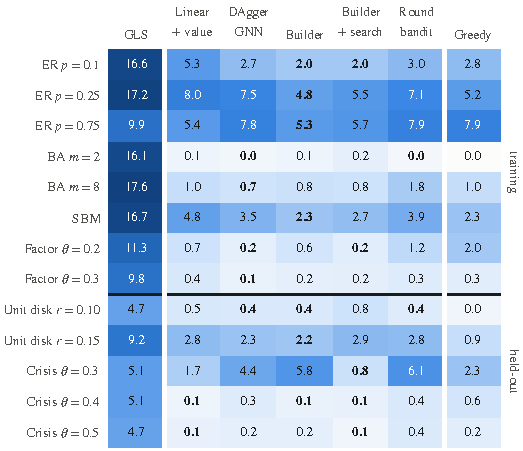
\includegraphics[width=\columnwidth]{figures/families.pdf}
\caption{Mean gap (\%) per setting on the fresh instances. Bold marks the lowest learned value in each row. Colour is on a square-root scale.}
\label{fig:families}
\end{figure}

\begin{figure*}[t]
\centering
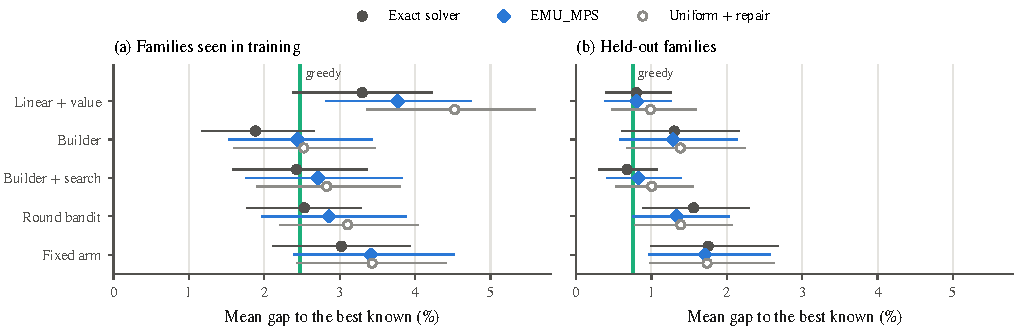
\includegraphics[width=\textwidth]{figures/emulator.pdf}
\caption{Whole decompositions on 156 fresh instances with each piece solved exactly (grey), sampled from \emumps{} (blue), or answered by random bitstrings and repair (open). Bars are $95\%$ intervals; the green line is min-degree greedy. \GLS{}, not shown, has gaps of $13.8$, $13.4$ and $14.2\%$ on training families and $5.9$, $5.6$ and $6.4\%$ on held-out families.}
\label{fig:emulator}
\end{figure*}

\GLS{} has the largest gap in every setting but one (Fig.~\ref{fig:families}). The learned methods beat greedy on dense Erd\H{o}s--R\'enyi graphs ($p=0.75$) and on calm market graphs at $\theta=0.2$, while greedy wins on unit-disk graphs, the one family that embeds well on the layout. The exception is the crisis market setting at $\theta = 0.3$, where the builder ($5.8\%$) and the round bandit ($6.1\%$) do worse than \GLS{} ($5.1\%$) and the DAgger GNN reaches $4.4\%$. All three rank pieces with the DAgger-trained GIN ranker or a policy-gradient refinement of it, while builder + search, which ranks with GraphSAGE, reaches $0.8\%$.

At $n = 300$, twice the largest training size, we ran ten test instances for each of two settings. The learned methods keep their lead over \GLS{} but fall behind greedy. On Erd\H{o}s--R\'enyi graphs with $p = 0.25$, builder + search reaches $8.6\%$ against $22.7\%$ for \GLS{} and $7.3\%$ for greedy, measured against best known rather than proven optima; on Barab\'asi--Albert graphs with $m=2$, greedy finds the optimum, the learned methods are within $0.6\%$, and \GLS{} is at $16.5\%$.

\section{Quantum-sampled pieces}
\label{sec:emulator}

The results above solve each piece exactly. A quantum processor returns samples instead, and a suboptimal sample changes every later decision. To test this, we ran whole decompositions with every piece solved on \emumps{}, Pasqal's tensor-network emulator~\cite{bidzhiev2025emulation}, on 156 fresh instances, for six methods: the four of Table~\ref{tab:fresh}, the round bandit, and the same stack with its per-round choice fixed at $(k, s, \text{beam}) = (2,2,2)$ (``fixed arm''). Pieces were compiled with Pulser on the \texttt{AnalogDevice} layout and channels, with its layout-filling limit lifted so that pieces of more than 30 atoms fit. They were driven for $4\,\mu$s by the annealing schedule in Pasqal's code~\cite{garrigues2025docking}, which is that of Refs.~\cite{cazals2025gadgets,cazals2025hard} except that the detuning starts at the channel limit, $-125.7$\,rad/$\mu$s, and sampled 500 times without noise. The same 936 decompositions were repeated with the exact solver and with a control that gives each piece 500 uniformly random bitstrings, repaired the same way. This took 15{,}201 emulator jobs.

The learned methods keep their lead over \GLS{}, about 10 points on training families and 4 to 5 on held-out ones (Fig.~\ref{fig:emulator}). Sampled answers raise the gap of the learned methods by 0.3 to 0.6 points on training families, though no single difference is clearly distinguishable from zero, and change nothing measurable on held-out families. \GLS{}, whose pieces are largest, does slightly better on the emulator.

The random control does about as well as the emulator. The reason is piece size: $92\%$ of solves have 15 atoms or fewer, where repaired random bitstrings are already near optimal and $98$ to $100\%$ of emulator shots are optimal. Only \GLS{} sends pieces above 30 atoms, where the share of optimal shots falls to $70\%$. So the learned methods do not depend on exact piece solutions, but at these sizes the quantum step adds nothing that random sampling does not.

\section{Conclusion}

Learned decisions make the \GLS{} decomposition much more accurate. On fresh instances the best models cut the gap of \GLS{} by a factor of six to seven, on held-out families as well as on those seen in training, and one of them does so with fewer quantum runs. The gains are smaller but persist on graphs twice the training size and with emulator-sampled pieces. Most of the gain comes from two cheap changes, ranking growth candidates with learned features and pruning branches by a predicted final size.

At these sizes, however, the decomposition is at best slightly better than classical min-degree greedy, and only on the families it was trained on, while the quantum step can be replaced by random sampling with repair. Both follow from how small the pieces on a 61-trap layout are. The learned methods should matter more on larger layouts, where the processor solves pieces that classical repair cannot and each quantum run is costly. Testing that requires larger devices and noisy hardware, which we did not use.

\begin{acknowledgments}
I thank Michael Haydock for supervising this work, and Pasqal for access to its cloud emulators. AI was utilized in the development of this project. The \GLS{} baseline reimplements Pasqal's open-source code, which is included unchanged in the repository under its licence and used to test the reimplementation.
\end{acknowledgments}

\textit{Code and data.} The code, trained models, every record behind the reported numbers, the saved emulator answers and the script that computes every number in this paper from them are at \url{https://github.com/hbofz/learned-gls}.

\appendix

\section{Pasqal's code and the published loop}
\label{app:code}

Pasqal's public \GLS{} code~\cite{garrigues2025docking} differs from the description in Ref.~\cite{cazals2025gadgets} in five ways. (i) It grows a piece from every vertex of the remaining graph and solves the $k$ largest, instead of growing $k$ pieces from random seeds. (ii) It places the first vertex on trap 32, on the edge of the layout [Fig.~\ref{fig:piece}(b)], not on the central trap. (iii) Its vertex score uses degree only; the number of already placed neighbours mentioned in the paper is not used. (iv) The parameter $\ell$ is a trigger, not a beam width: the beam is pruned to $k$ branches only when a running count of solved children exceeds $\ell$. At $(4,2,10)$ the code therefore solves 16 pieces per round in steady state, four for each of four branches, against 40 for the published loop with its ten branches. (v) A fixed random seed inside every mapping makes repeated runs identical. On the test seeds, the code's loop exceeded 1000 branches on a third of the training-family instances and more than half of the held-out ones, which is why we bound it. Our reconstruction of the published loop (random seeds, central trap, a beam of $\ell$ branches), which keeps the code's degree-only score, has gaps of $13.1\%$ and $5.0\%$ on the test seeds at more than twice the runs of the bounded loop.

\bibliography{refs}

\end{document}
